\documentclass[11pt]{article}

\usepackage[margin=1in]{geometry}
\usepackage{booktabs}
\usepackage{graphicx}
\usepackage{float}
\usepackage{hyperref}

\title{Matrix Benchmark Timing Report}
\author{Codex benchmark sweep for the Matrix project}
\date{March 15, 2026}

\begin{document}

\maketitle

\section{Benchmark Setup}
This report summarizes a quick but broad timing sweep for the four shipped test
programs: matrix multiplication, REF, RREF, and LU. The benchmark data was
generated by \texttt{benchmarks/scripts/run\_benchmarks.py} and written to
\texttt{benchmarks/data/timings.csv} and \texttt{benchmarks/data/summary.csv}.

\begin{itemize}
\item Matrix sizes: $250$, $500$, $1000$, and $1500$
\item MPI process counts: $1$, $2$, $4$, $8$, and $16$
\item Machine: $32$ logical CPU cores, about $24$ GiB of available RAM at run time
\item Timing source: kernel timings printed by the test executables themselves
\end{itemize}

The goal of this sweep was to stay fast enough to rerun easily while still
capturing how scaling changes across several problem sizes. These timings are
not intended to represent the maximum matrix size now supported by the heap
backed matrix implementation.

\section{Best Timing Summary}
\begin{table}[H]
\centering
\small
\begin{tabular}{rrrrrr}
\toprule
Operation & $N$ & Seq. (s) & Best MPI np & Best MPI (s) & Speedup \\
\midrule
LU & 250 & 0.005 & 4 & 0.005 & 1.00 \\
LU & 500 & 0.045 & 2 & 0.040 & 1.13 \\
LU & 1000 & 0.332 & 1 & 0.327 & 1.02 \\
LU & 1500 & 1.187 & 8 & 1.123 & 1.06 \\
Multiply & 250 & 0.017 & 8 & 0.004 & 4.25 \\
Multiply & 500 & 0.141 & 8 & 0.037 & 3.81 \\
Multiply & 1000 & 1.341 & 8 & 0.385 & 3.48 \\
Multiply & 1500 & 5.153 & 16 & 1.391 & 3.70 \\
REF & 250 & 0.006 & 4 & 0.003 & 2.00 \\
REF & 500 & 0.057 & 8 & 0.016 & 3.56 \\
REF & 1000 & 0.440 & 8 & 0.063 & 6.98 \\
REF & 1500 & 1.670 & 8 & 0.206 & 8.11 \\
RREF & 250 & 0.025 & 2 & 0.003 & 8.33 \\
RREF & 500 & 0.097 & 8 & 0.014 & 6.93 \\
RREF & 1000 & 0.781 & 8 & 0.087 & 8.98 \\
RREF & 1500 & 3.058 & 8 & 0.208 & 14.70 \\
\bottomrule
\end{tabular}
\caption{Best observed MPI kernel time at each benchmarked matrix size.}
\end{table}

\section{Observations}
\begin{itemize}
\item Matrix multiplication scaled well through \texttt{np=8} and remained strong at \texttt{np=16}. The best observed result was $1.391$ seconds at $N=1500$ with \texttt{np=16}, compared with $5.153$ seconds sequential.
\item REF showed its best results at \texttt{np=8} for the three larger sizes. At $N=1500$, the best MPI run was $0.206$ seconds versus $1.670$ seconds sequential, which is about an $8.11\times$ speedup.
\item RREF produced the strongest scaling in this sweep. At $N=1500$, the best MPI timing was $0.208$ seconds at \texttt{np=8}, compared with $3.058$ seconds sequential, a speedup of about $14.70\times$.
\item LU remained effectively sequential in practice. The current test harness only performs the decomposition on rank $0$, so additional MPI processes mostly add launch and synchronization overhead rather than real distributed compute.
\item The raw wall times in \texttt{timings.csv} are much larger than the kernel times for small matrices because \texttt{mpirun} startup dominates those runs. The kernel timings are the correct numbers to use when comparing the algorithm implementations inside the existing test drivers.
\end{itemize}

\section{Figures}
\begin{figure}[H]
\centering
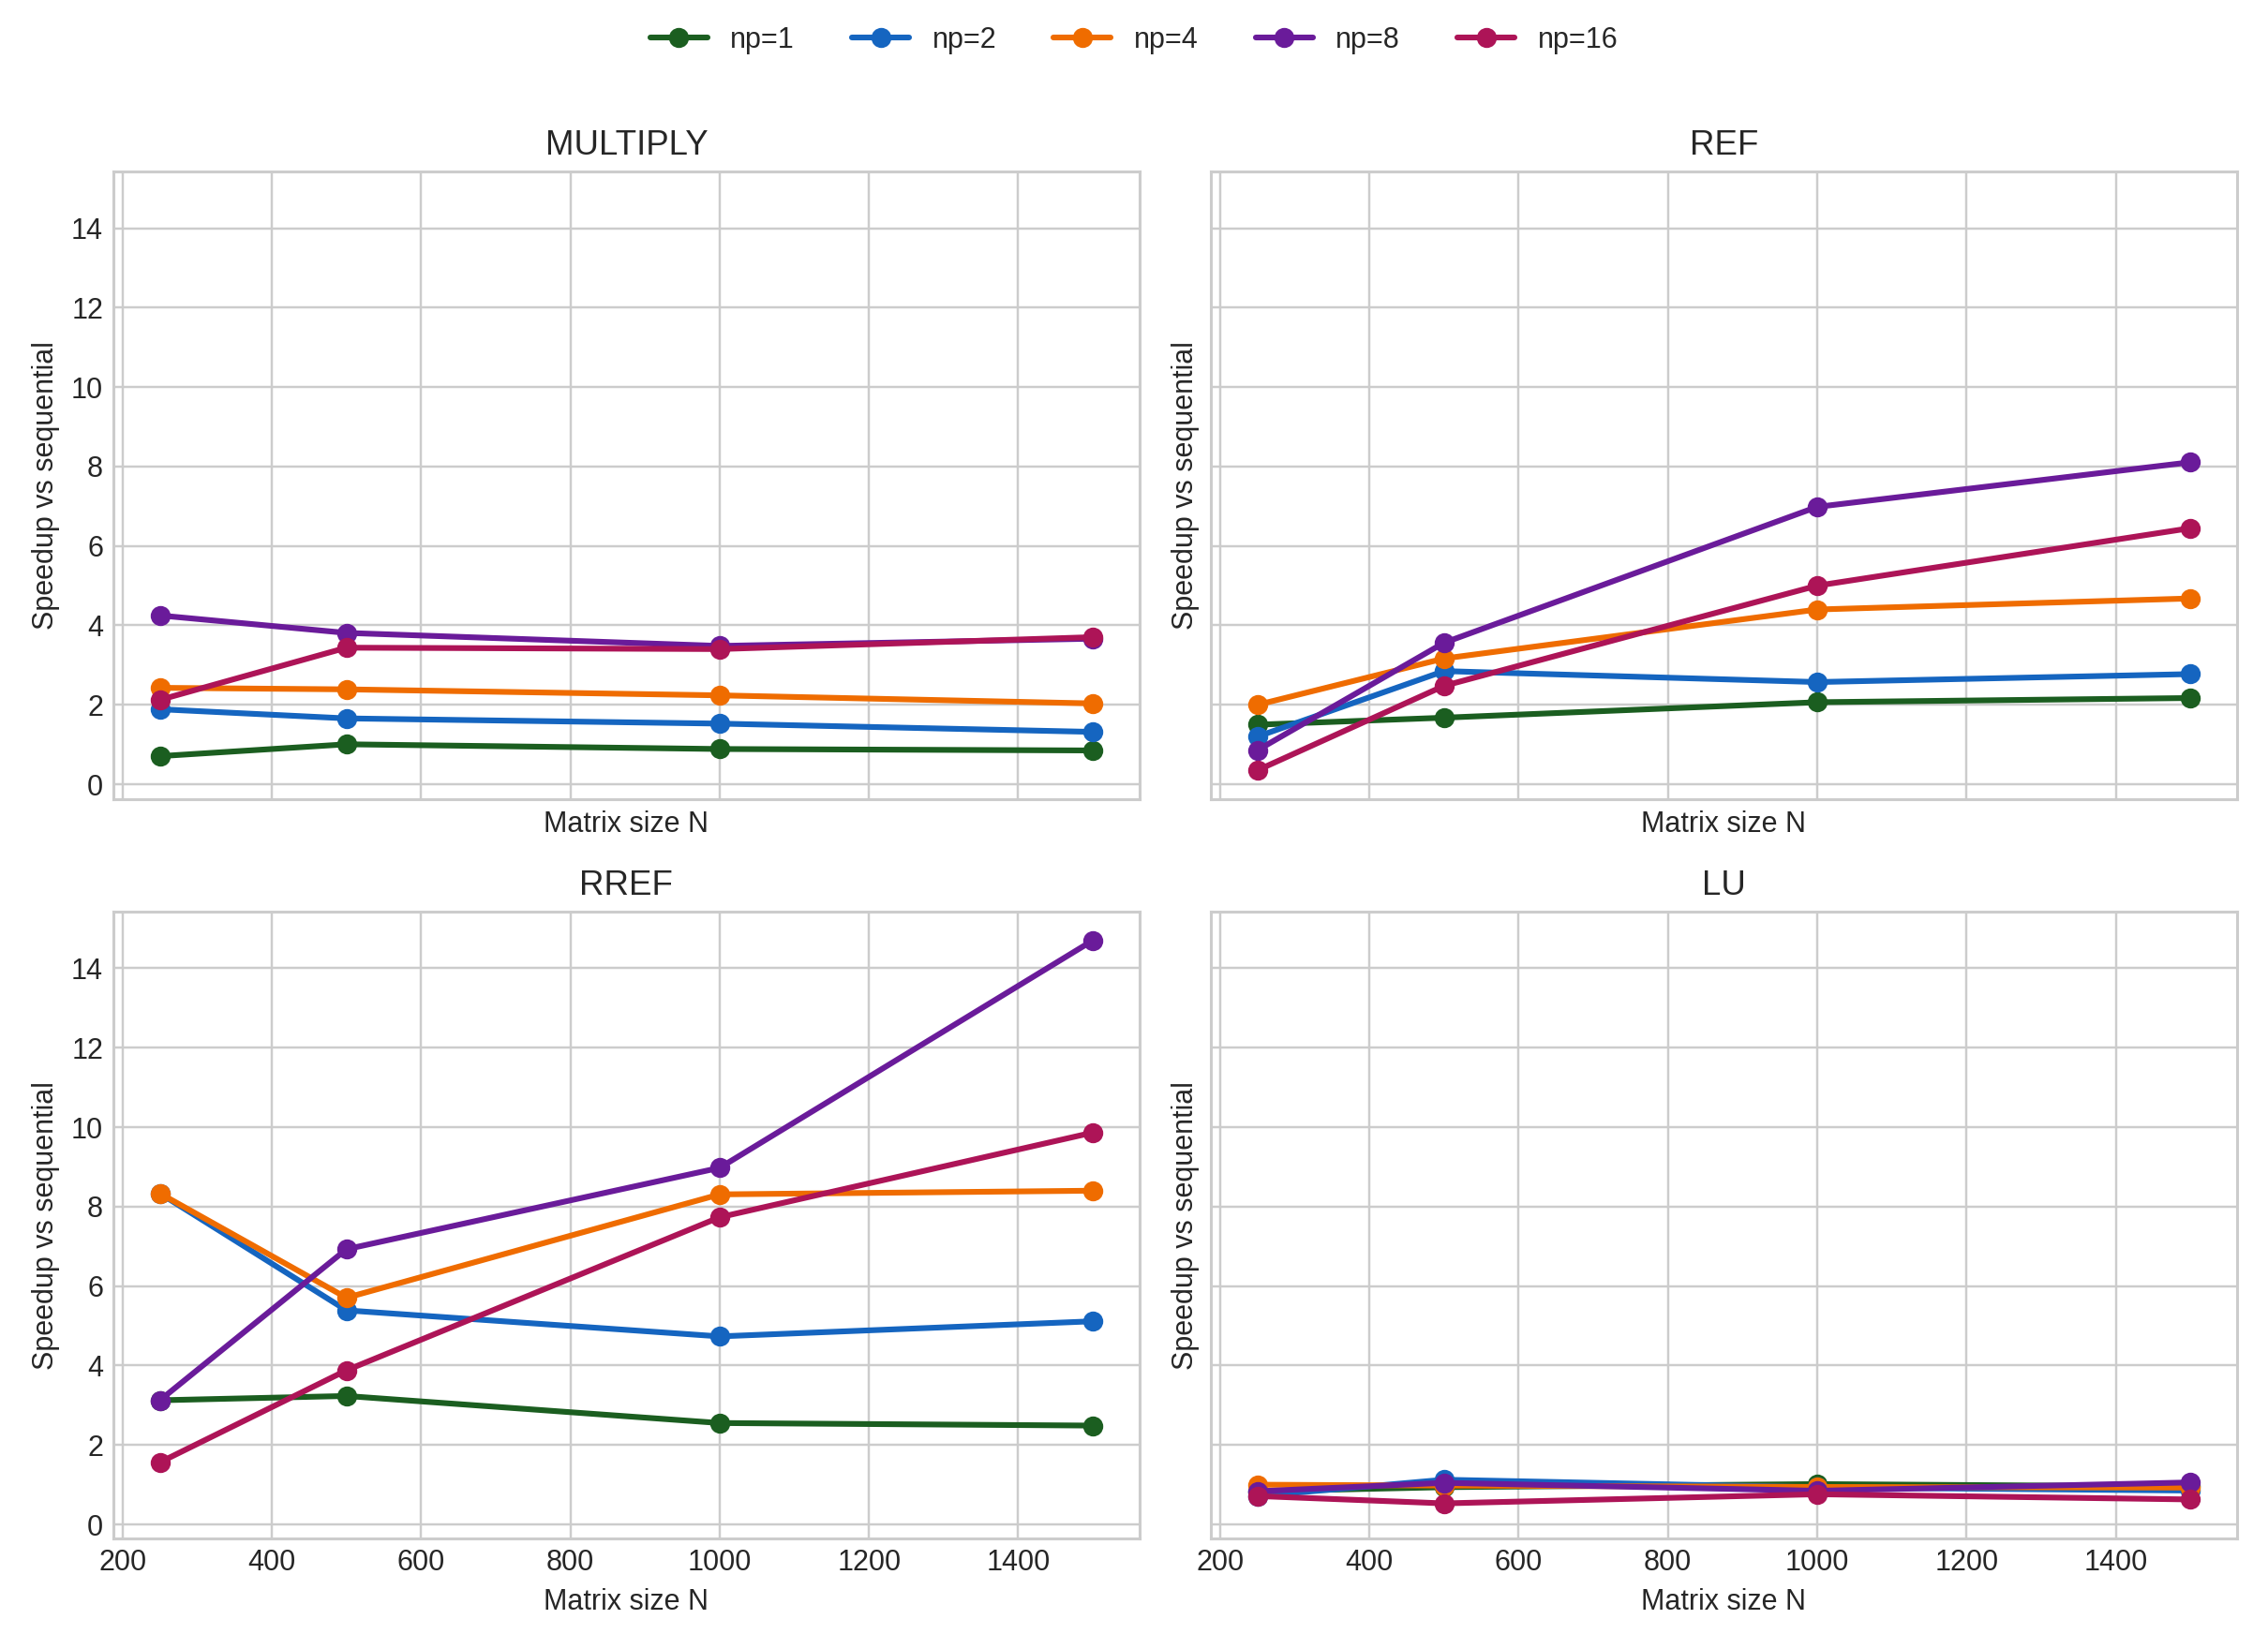
\includegraphics[width=0.95\textwidth]{../figures/speedup_summary.png}
\caption{Speedup relative to the sequential baseline across all four operations.}
\end{figure}

\begin{figure}[H]
\centering
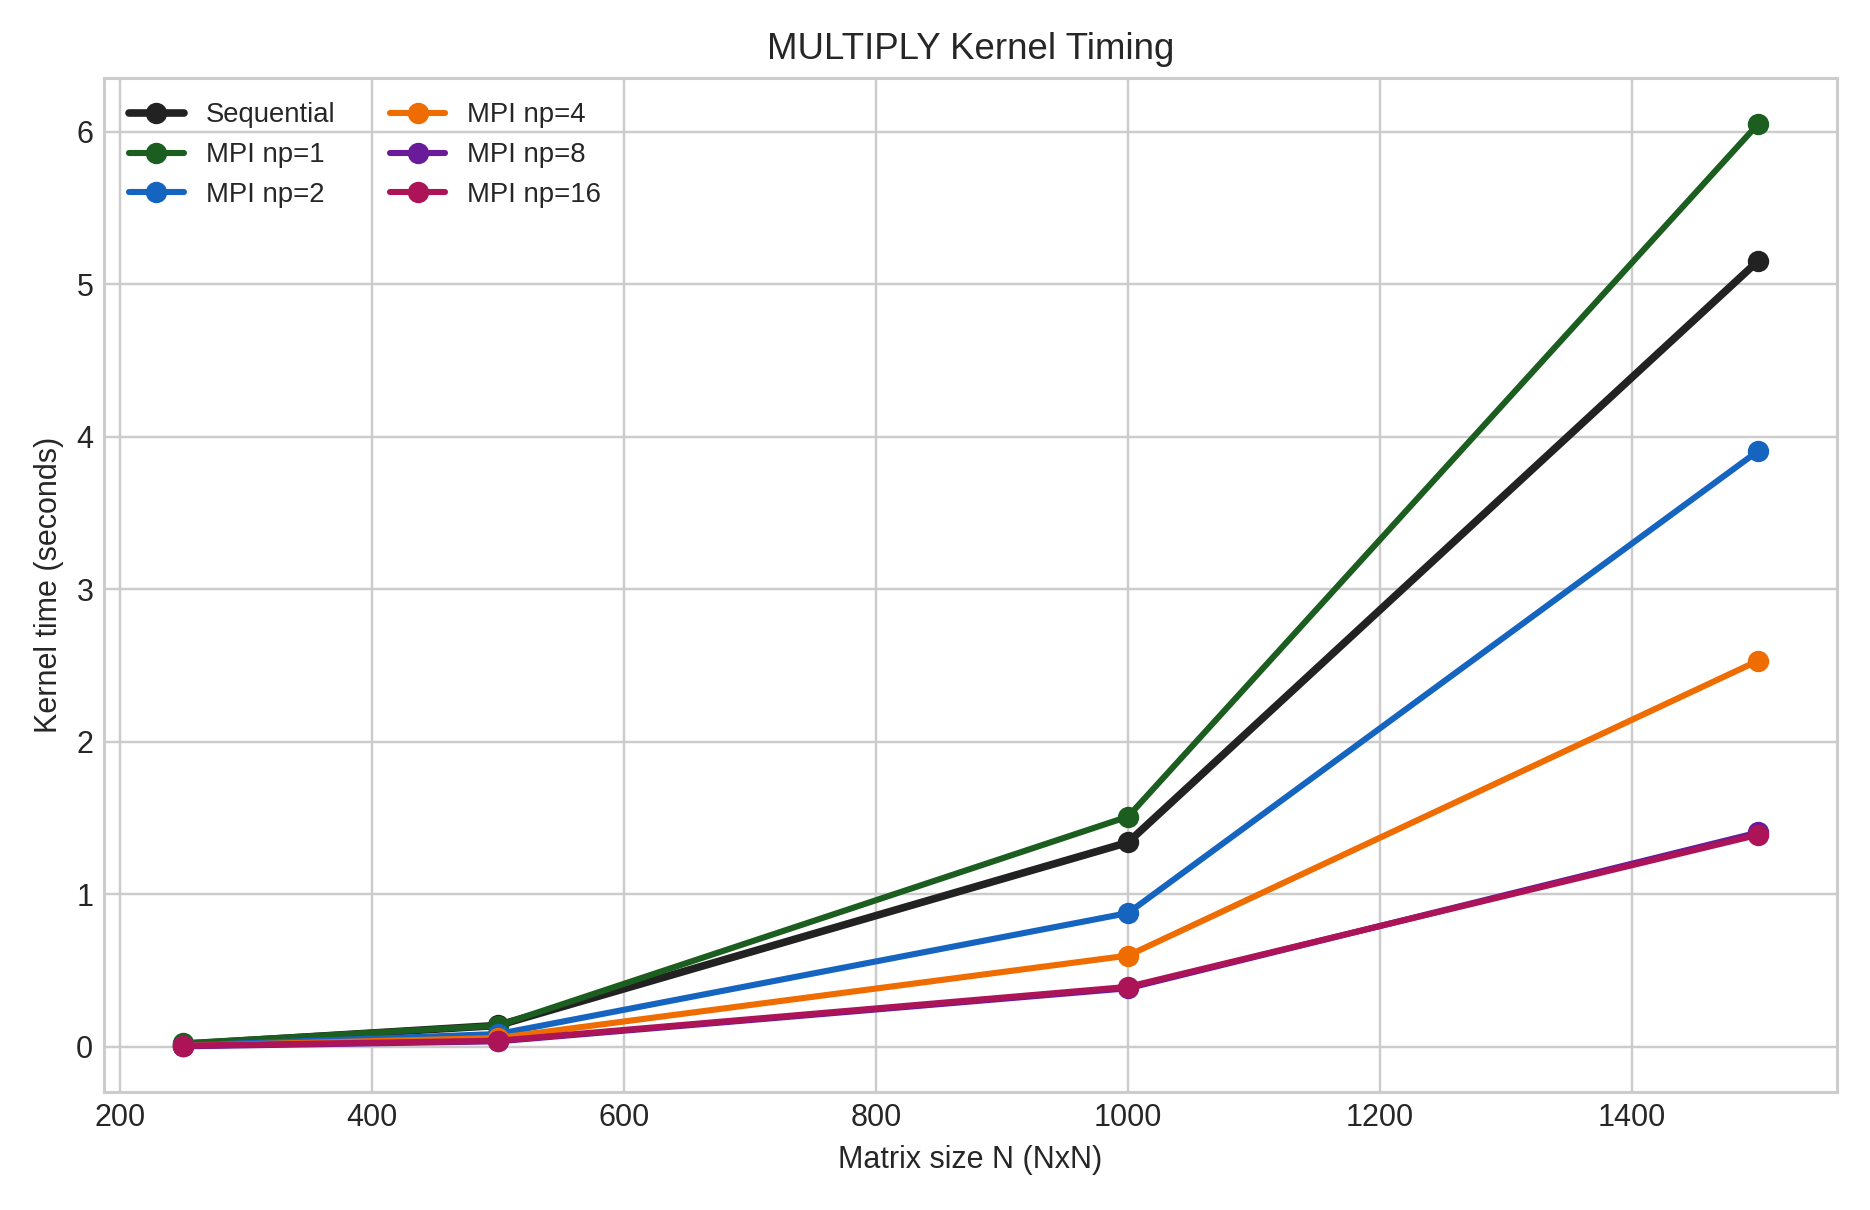
\includegraphics[width=0.9\textwidth]{../figures/multiply_timing.png}
\caption{Matrix multiplication kernel timings across process counts.}
\end{figure}

\begin{figure}[H]
\centering
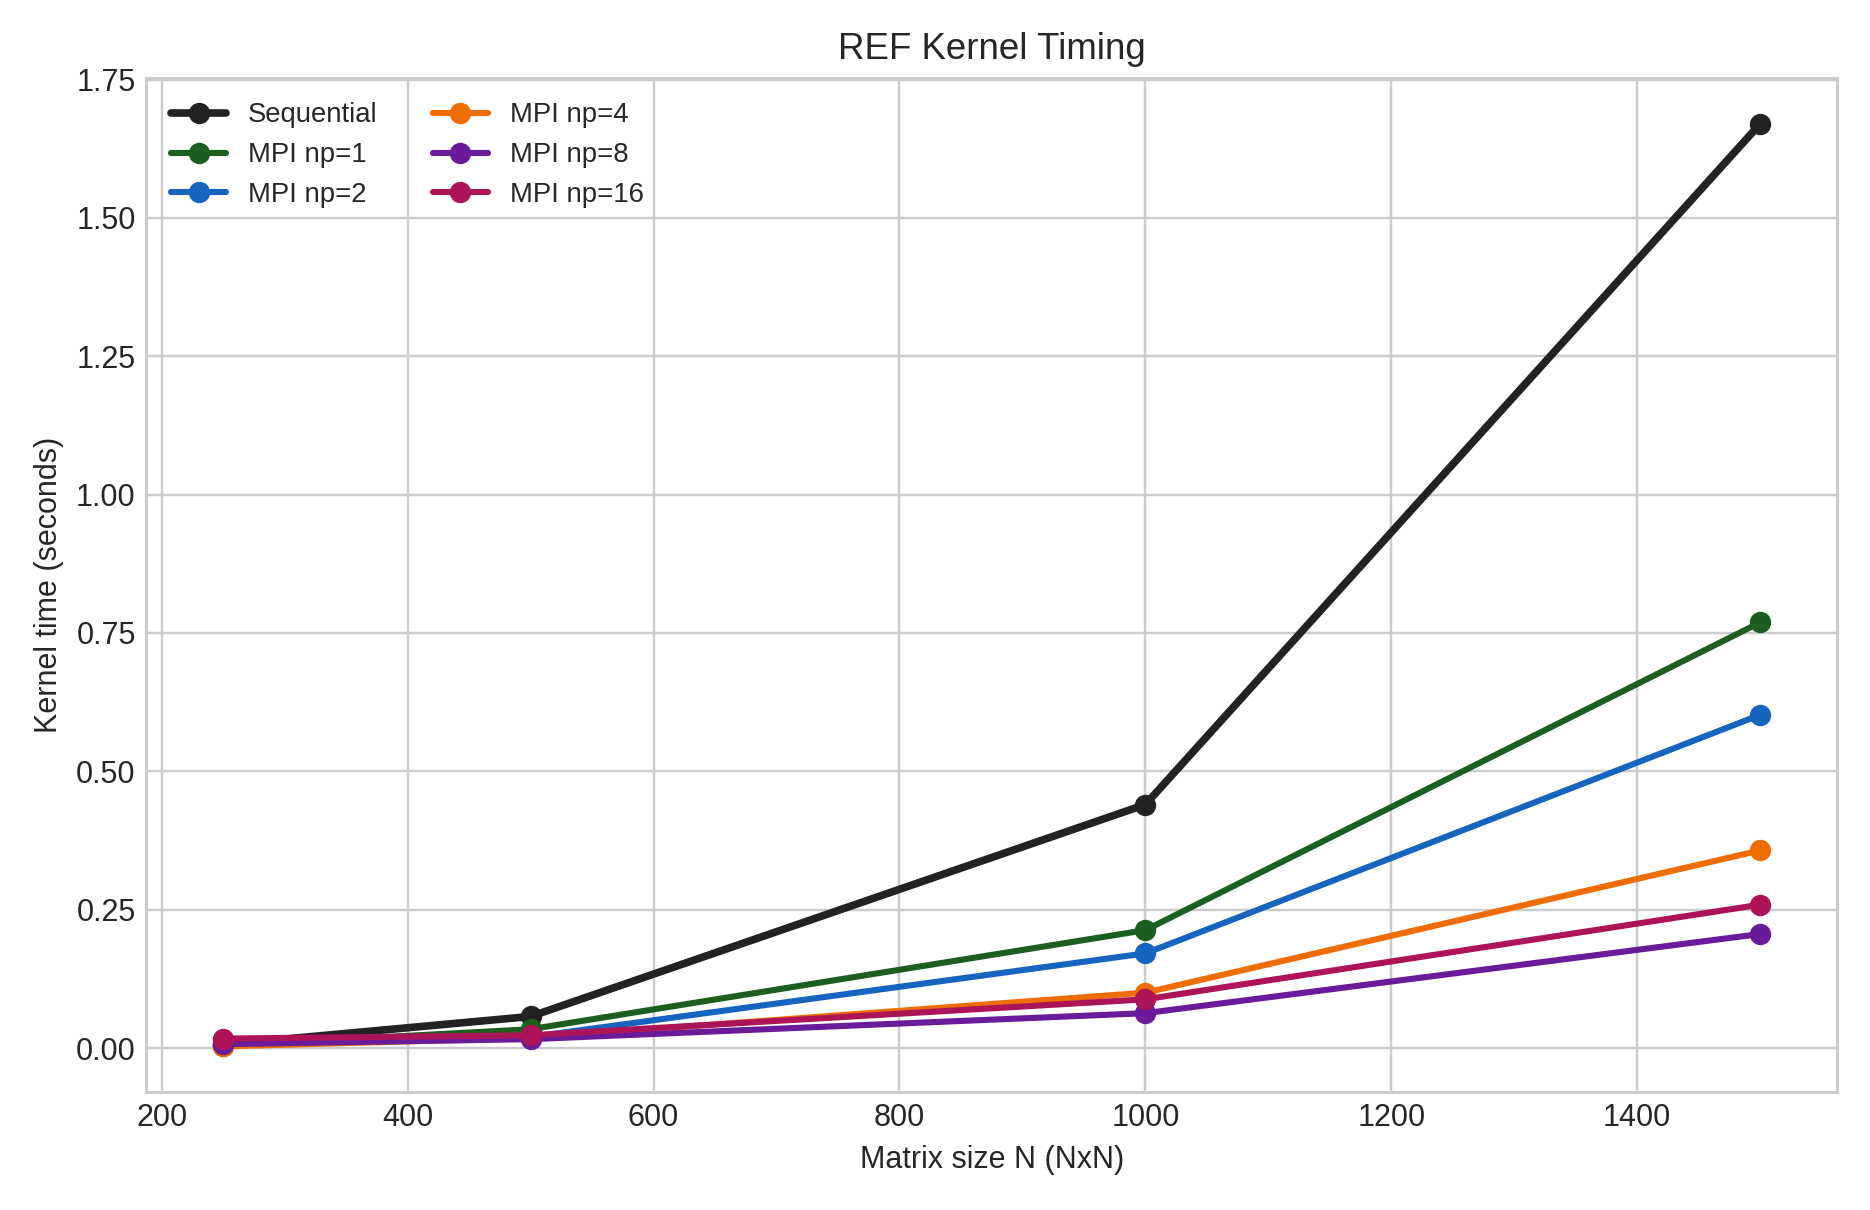
\includegraphics[width=0.9\textwidth]{../figures/ref_timing.png}
\caption{REF kernel timings across process counts.}
\end{figure}

\begin{figure}[H]
\centering
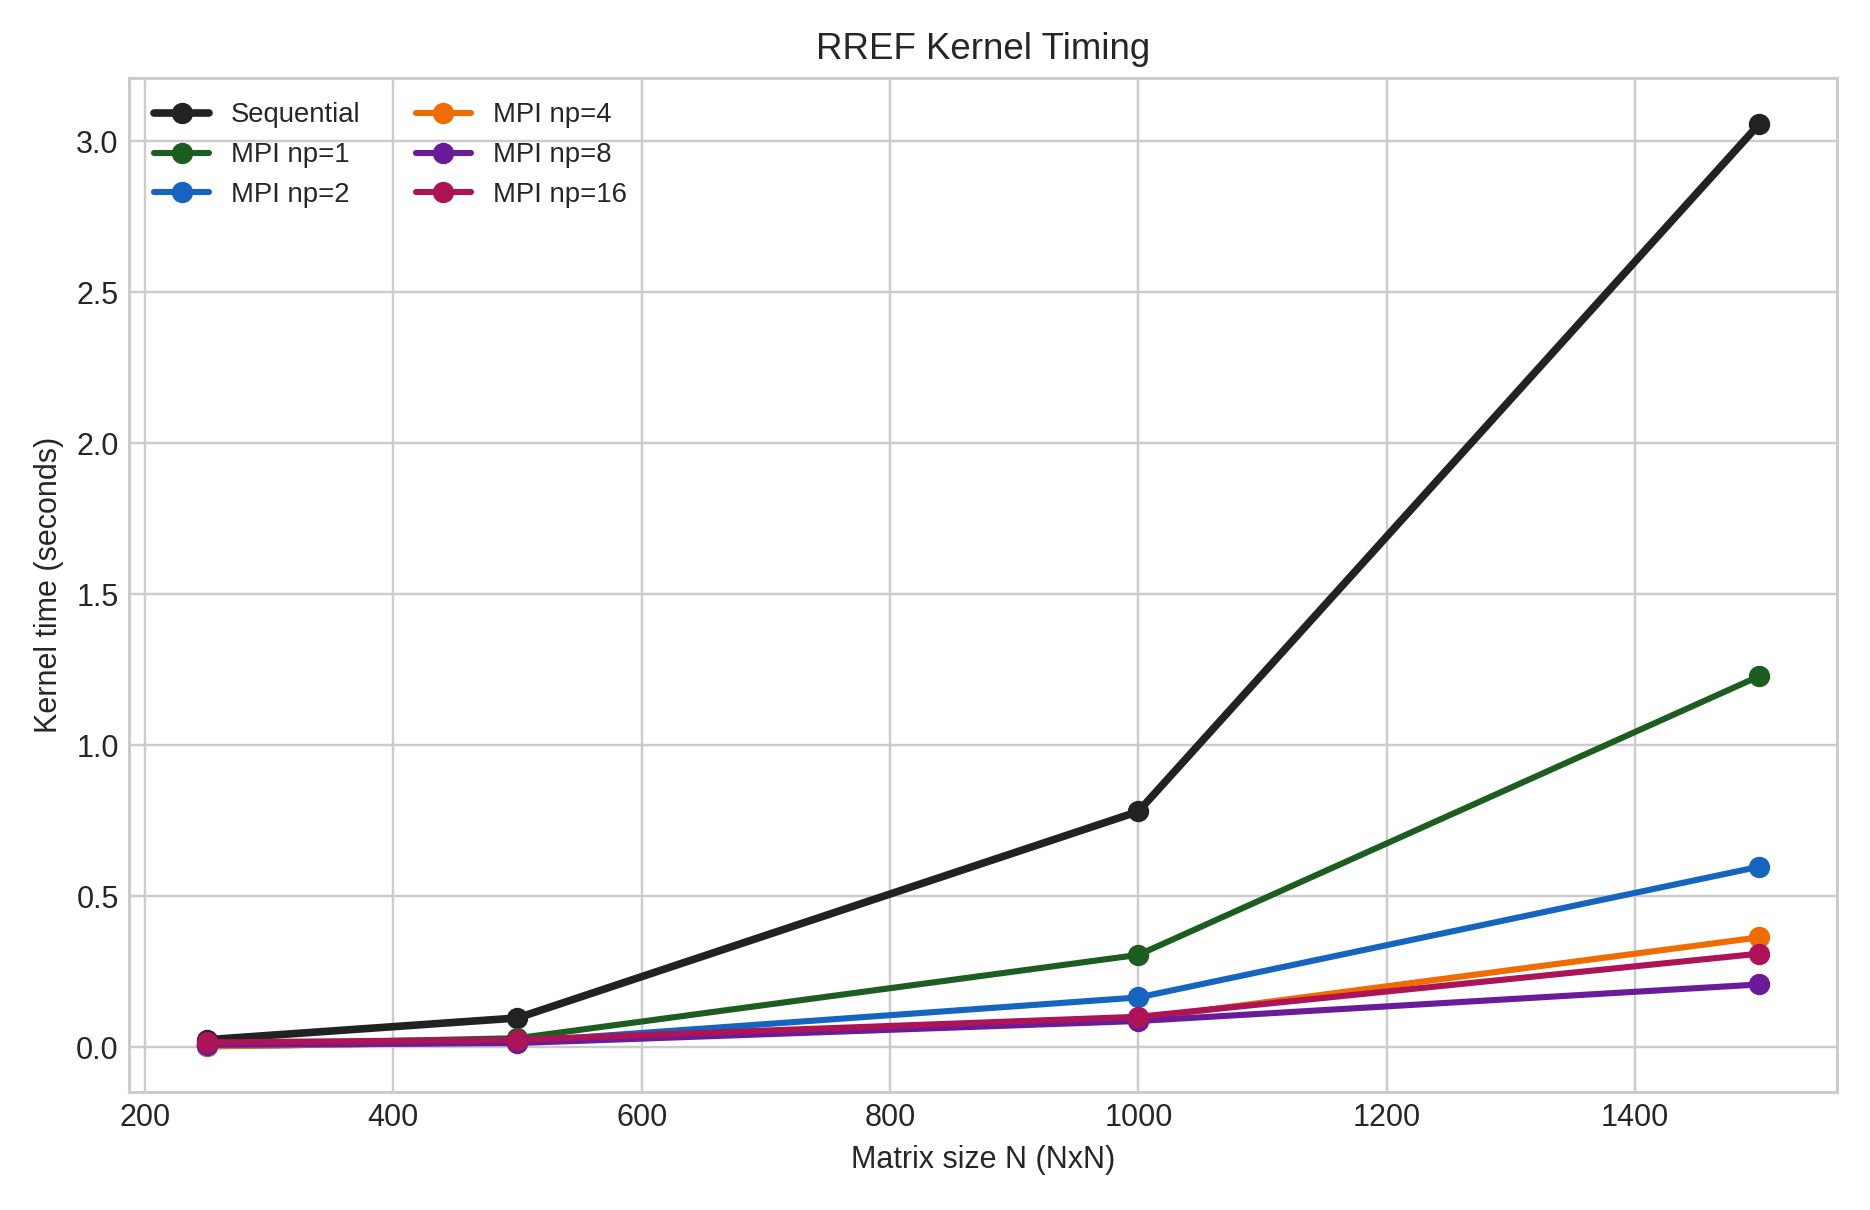
\includegraphics[width=0.9\textwidth]{../figures/rref_timing.png}
\caption{RREF kernel timings across process counts.}
\end{figure}

\begin{figure}[H]
\centering
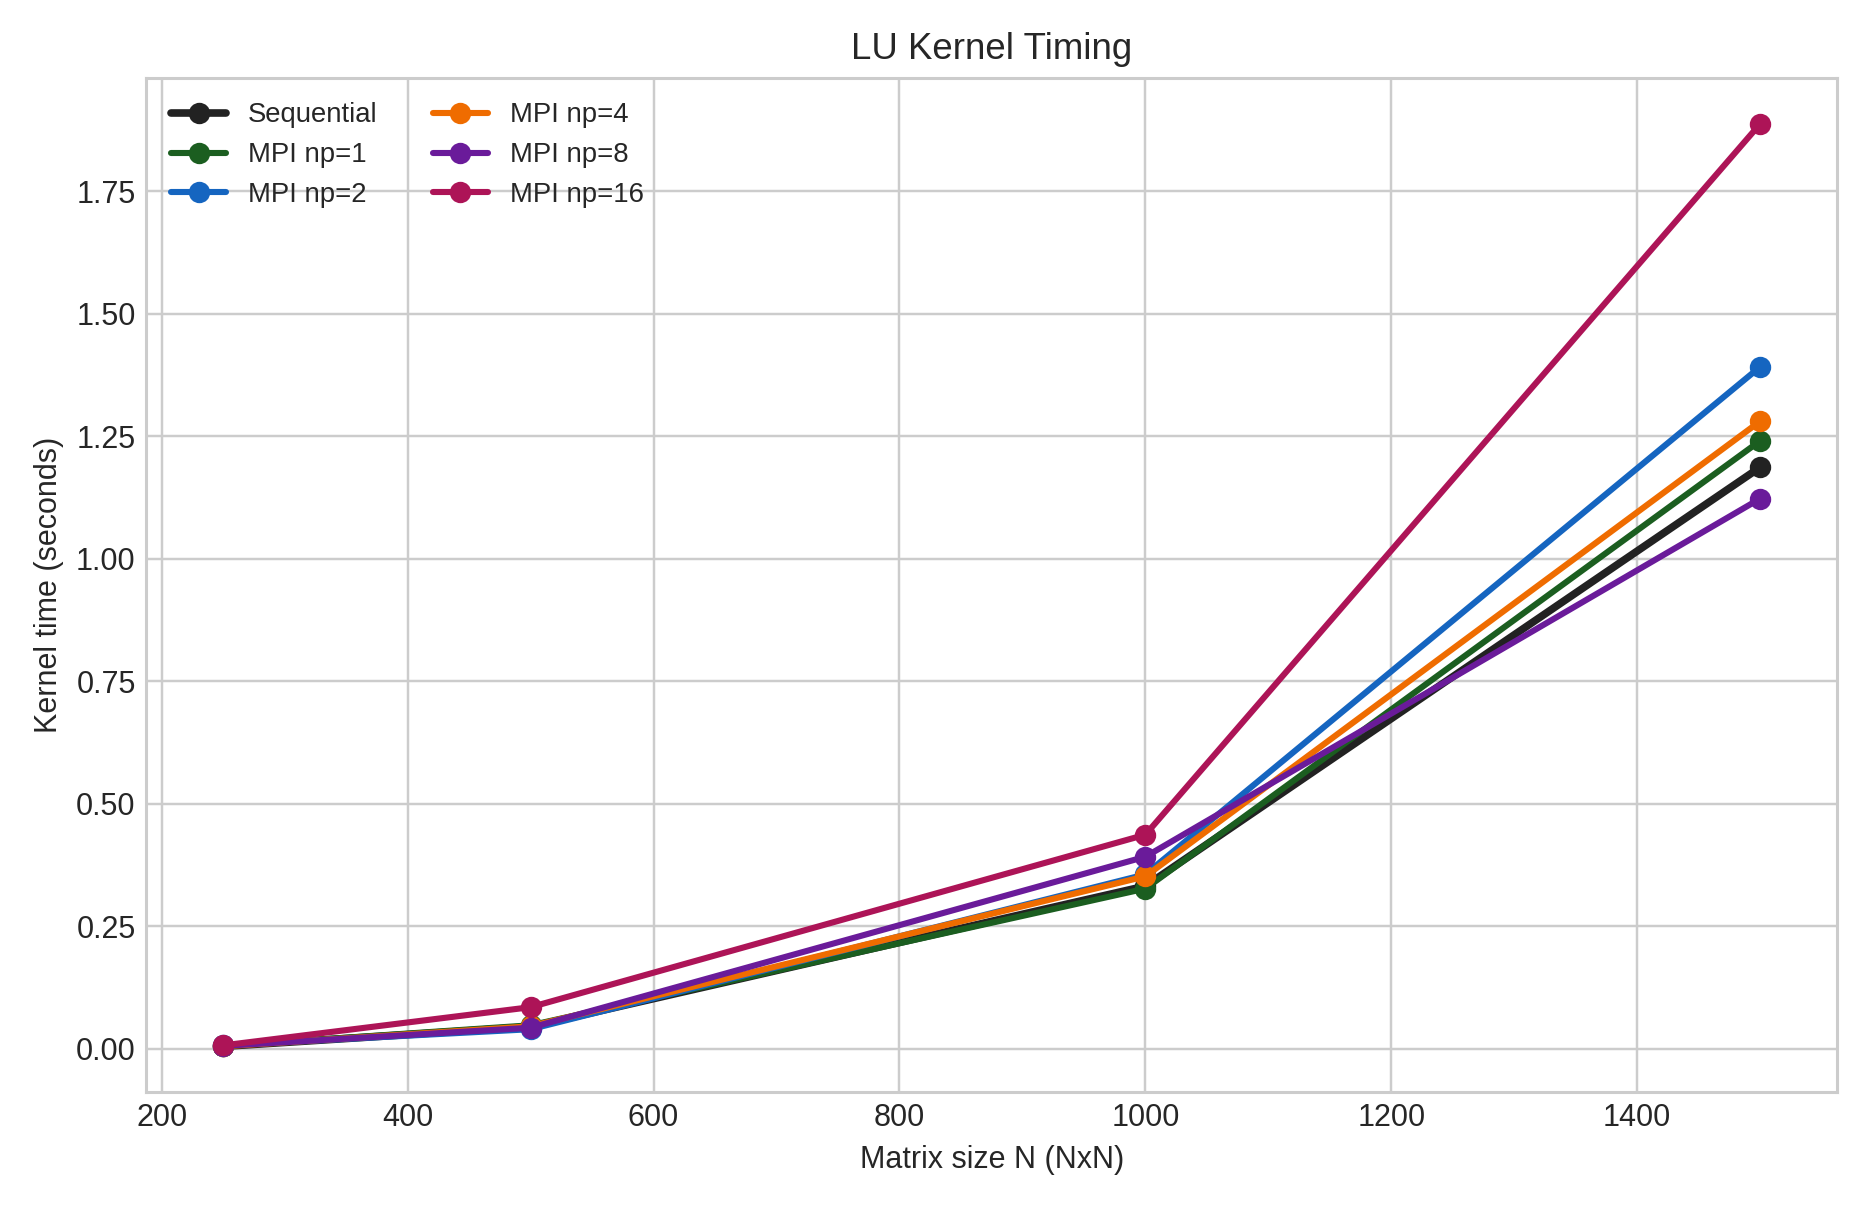
\includegraphics[width=0.9\textwidth]{../figures/lu_timing.png}
\caption{LU kernel timings across process counts.}
\end{figure}

\section{Conclusion}
This benchmark sweep confirms a clear split in behavior across the current
implementations. Matrix multiplication, REF, and RREF all benefit from
additional MPI ranks on the tested sizes, with RREF showing the strongest
measured speedups. LU does not currently show comparable scaling because it is
still executed only on rank $0$ in the test harness. As a result, the new heap
backed matrix storage removes the old size cap, but LU still needs a true
distributed algorithm before higher MPI process counts will help materially.

\end{document}
